\documentclass{article}

% Pacchetti utili
\usepackage[utf8]{inputenc} % Per la codifica dei caratteri
\usepackage[T1]{fontenc} % Per i font
\usepackage{graphicx} % Per le immagini
\usepackage{amsmath, amssymb} % Per la matematica
\usepackage{hyperref} % Per i link
\usepackage{natbib} % Per le citazioni
\usepackage{algorithm}
\usepackage{algorithmicx}
\usepackage{algpseudocode}
\usepackage{amsmath}
\usepackage{amsfonts}


\begin{document}

Gli \textit{item} e le \textit{query} vengono mappati su  vettore di \textit{embedding} in uno spazio comune $E = \mathbb{R}^k$. Normalmente lo spazio di \textit{embedding} ha una dimensione molto più piccola rispetto alla grandezza del corpus e cattura alcune strutture latenti dell'insieme di \textit{item} o \textit{query}. Gli elementi tra loro simili finiscono per essere vicini nello spazio di \textit{embedding}. Il concetto di "vicinanza" è definito da una misura di similarità.
 
Una misura di similarità è una funzione $s: E \times E \to \mathbb{R}$ che prende in input una coppia di vettori di \textit{embedding} e restituisce un valore scalare che ne misura la similarità. Gli \textit{embedding} possono essere utilizzati per la generazione dei candidati come segue: dato un vettore di \textit{embedding} per una query $q \in E$, il sistema cerca gli \textit{embedding} degli elementi $x \in E$ che sono vicini a $q$, ossia, gli \textit{embedding} con una similarità elevata.

Per determinare il grado di similarità, la maggior parte dei sistemi di \textit{recommendation} si basa su una o più delle seguenti misure:

\begin{itemize}
    \item coseno: semplicemente il coseno dell'angolo tra i due vettori $s(q, x) = cos(q, x)$
    \item prodotto scalare: è dato da: $s(q, x) = \langle q, x \rangle = \sum\limits_{i=1}^{d} q_i x_i$. È anche dato da $s(q, x) = \|x\| \|q\| \cos(q, x)$ che corrisponde al coseno dell'angolo moltiplicato per il prodotto delle norme. Pertanto, se gli \textit{embedding} sono normalizzati, il prodotto scalare e il coseno coincidono    
    \item distanza euclidea: questa è la distanza usuale nello spazio euclideo $s(q, x) = \|q - x\| = \left[ \sum\limits_{i=1}^{d} (q_i - x_i)^2 \right]^{\frac{1}{2}}$. Una distanza minore indica una similarità maggiore. Da notare che, quando gli \textit{embedding} sono normalizzati, la distanza euclidea al quadrato coincide con il prodotto scalare (e il coseno) fino a una costante, poiché in quel caso $\frac{1}{2} \|q - x\|^2 = 1 - \langle q, x \rangle$
\end{itemize}


\begin{figure}[H]
    \centering
    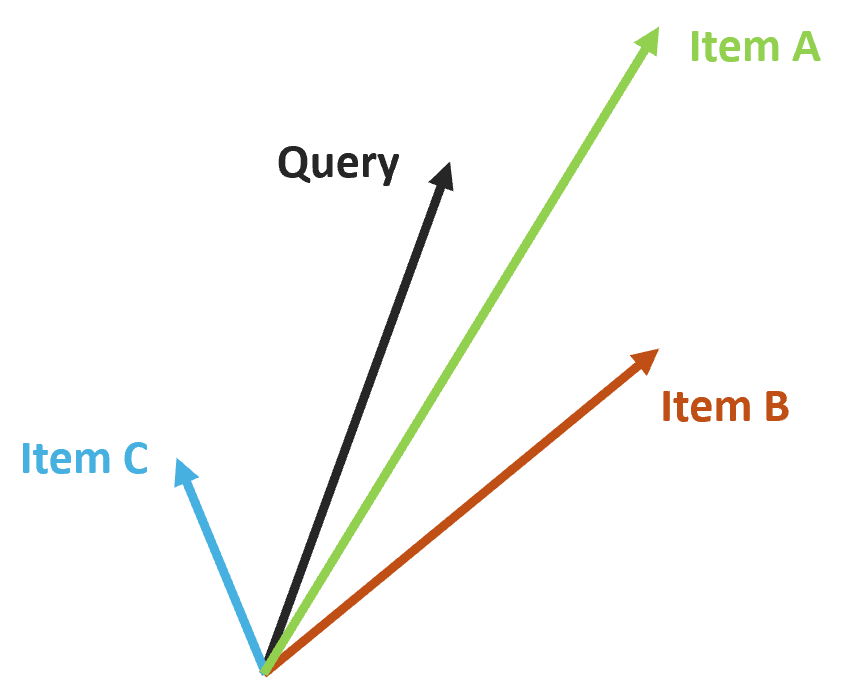
\includegraphics[scale=0.8]{../figures/embedding.PNG}
    \caption{Il vettore nero illustra l'\textit{embedding} della query. Gli altri tre vettori di \textit{embedding} (\textit{Item A}, \textit{Item B}, \textit{Item C}) rappresentano gli \text{item} candidati. A seconda della misura di similarità utilizzata, la classifica degli elementi può essere diversa}
    \label{fig:embedding}
\end{figure}

Rispetto al coseno, la similarità del prodotto scalare è sensibile alla norma dell'\textit{embedding}. Cioè, maggiore è la norma di un \textit{embedding}, maggiore sarà la similarità e più è probabile che l'elemento venga raccomandato. Questo può influenzare le raccomandazioni nei seguenti modi:

\begin{itemize}
    \item gli elementi che appaiono molto frequentemente nel \textit{training set} (ad esempio, le top canzoni italiane del momento su \textit{Spotify}) tendono ad avere \textit{embedding} con norme grandi. Se è desiderabile catturare informazioni sulla popolarità, allora si dovrebbe preferire il prodotto scalare. Tuttavia, se non si presta attenzione, gli elementi popolari potrebbero finire per dominare le raccomandazioni. In pratica, si possono utilizzare altre varianti delle misure di similarità che pongono meno enfasi sulla norma dell'elemento. Ad esempio, definire $s(q, x) = \|q\|^{\alpha} \|x\|^{\alpha} \cos(q, x)$ per qualche $\alpha \in (0,1)$
    \item Gli elementi che appaiono molto raramente potrebbero non essere aggiornati frequentemente durante l'addestramento. Di conseguenza, se vengono inizializzati con una norma elevata, il sistema potrebbe raccomandare elementi rari invece di quelli più rilevanti. Per evitare questo problema, prestare attenzione all'inizializzazione degli \textit{embedding} e utilizzare una regolarizzazione appropriata
\end{itemize}





\bibliographystyle{plain}
\bibliography{../bibliography}

\end{document}
